\documentclass[9pt, aspectratio=169, handout]{beamer}

% +==================================================+
% |   ████████╗██╗  ██╗███████╗███╗   ███╗███████╗   |
% |   ╚══██╔══╝██║  ██║██╔════╝████╗ ████║██╔════╝   |
% |      ██║   ███████║█████╗  ██╔████╔██║█████╗     |
% |      ██║   ██╔══██║██╔══╝  ██║╚██╔╝██║██╔══╝     |
% |      ██║   ██║  ██║███████╗██║ ╚═╝ ██║███████╗   |
% |      ╚═╝   ╚═╝  ╚═╝╚══════╝╚═╝     ╚═╝╚══════╝   |
% +==================================================+

\useinnertheme{rectangles}
\useoutertheme{infolines}

\setbeamertemplate{footline}{%
    \leavevmode%
    \rule{\paperwidth}{0.1pt}\vskip0.2pt%
    \hbox{%
        \begin{beamercolorbox}[wd=.2\paperwidth, ht=2.25ex, dp=1ex, center]{author in head/foot}%
            \usebeamerfont{author in head/foot}\insertshortauthor
        \end{beamercolorbox}%
        \begin{beamercolorbox}[wd=.6\paperwidth, ht=2.25ex, dp=1ex, center]{title in head/foot}%
            \usebeamerfont{title in head/foot}\insertshorttitle
        \end{beamercolorbox}%
        \begin{beamercolorbox}[wd=.2\paperwidth, ht=2.25ex, dp=1ex, center]{date in head/foot}%
            \usebeamerfont{date in head/foot}\insertshortdate\hfill\insertframenumber{} / \inserttotalframenumber\hspace*{2ex}
        \end{beamercolorbox}%
    }%
    \vskip0pt%
}
% hrule under the frametitle, see:
% https://tex.stackexchange.com/questions/343517/beamer-full-width-hrule-below-frame-title
\setbeamertemplate{frametitle}{%
    \usebeamerfont{frametitle}\insertframetitle%
    \vphantom{g}%
    \par%
    \makebox[\linewidth][c]{%
        \rule[0.5\baselineskip]{\paperwidth}{0.4pt}%
    }%
}

% \beamertemplatenavigationsymbolsempty % remove navigation bar

\definecolor{grey80}{HTML}{CCCCCC}
\definecolor{grey90}{HTML}{E6E6E6}
\definecolor{grey95}{HTML}{F2F2F2}

\usepackage[svgnames, x11names]{xcolor}
\usecolortheme[named=DarkSlateGrey]{structure}
\setbeamercolor{background canvas}{bg=white}

\setbeamerfont{frametitle}{series=\bfseries}

\let\oldtiny\tiny
\let\oldscriptsize\scriptsize
\let\oldfootnotesize\footnotesize
\let\oldsmall\small
\let\oldnormalsize\normalsize
\let\oldlarge\large
\let\oldLarge\Large
\let\oldLARGE\LARGE
\let\oldhuge\huge
\let\oldHuge\Huge
\renewcommand*{\footnotesize}{\oldfootnotesize\scriptsize}
\renewcommand*{\normalsize}{\oldnormalsize\oldsmall}
\setbeamerfont{frametitle}{size=\oldnormalsize}

% +=================================+
% |   ██████╗ ██╗██████╗ ███████╗   |
% |   ██╔══██╗██║██╔══██╗██╔════╝   |
% |   ██████╔╝██║██████╔╝███████╗   |
% |   ██╔══██╗██║██╔══██╗╚════██║   |
% |   ██████╔╝██║██████╔╝███████║   |
% |   ╚═════╝ ╚═╝╚═════╝ ╚══════╝   |
% +=================================+

% \usepackage[style=nejm,backend=biber]{biblatex}
% \addbibresource{my.bib}
% \renewcommand*{\bibfont}{\footnotesize}

% +==========================================+
% |   ███╗   ███╗ █████╗ ████████╗██╗  ██╗   |
% |   ████╗ ████║██╔══██╗╚══██╔══╝██║  ██║   |
% |   ██╔████╔██║███████║   ██║   ███████║   |
% |   ██║╚██╔╝██║██╔══██║   ██║   ██╔══██║   |
% |   ██║ ╚═╝ ██║██║  ██║   ██║   ██║  ██║   |
% |   ╚═╝     ╚═╝╚═╝  ╚═╝   ╚═╝   ╚═╝  ╚═╝   |
% +==========================================+

\usepackage{amsmath,amssymb,amsfonts}
\usepackage{cancel}
\usepackage{braket}
\usepackage{bm}
\usepackage{siunitx}
\usepackage{feynmf}
\usepackage{cleveref}
\DeclareGraphicsRule{*}{mps}{*}{}

% +===================================================+
% |   ███████╗██╗ ██████╗ ██╗   ██╗██████╗ ███████╗   |
% |   ██╔════╝██║██╔════╝ ██║   ██║██╔══██╗██╔════╝   |
% |   █████╗  ██║██║  ███╗██║   ██║██████╔╝█████╗     |
% |   ██╔══╝  ██║██║   ██║██║   ██║██╔══██╗██╔══╝     |
% |   ██║     ██║╚██████╔╝╚██████╔╝██║  ██║███████╗   |
% |   ╚═╝     ╚═╝ ╚═════╝  ╚═════╝ ╚═╝  ╚═╝╚══════╝   |
% +===================================================+
\usepackage{subcaption}
\usepackage{makecell}
\usepackage{booktabs}

% +===========================================================+
% |    ██████╗██╗  ██╗██╗███╗   ██╗███████╗███████╗███████╗   |
% |   ██╔════╝██║  ██║██║████╗  ██║██╔════╝██╔════╝██╔════╝   |
% |   ██║     ███████║██║██╔██╗ ██║█████╗  ███████╗█████╗     |
% |   ██║     ██╔══██║██║██║╚██╗██║██╔══╝  ╚════██║██╔══╝     |
% |   ╚██████╗██║  ██║██║██║ ╚████║███████╗███████║███████╗   |
% |    ╚═════╝╚═╝  ╚═╝╚═╝╚═╝  ╚═══╝╚══════╝╚══════╝╚══════╝   |
% +===========================================================+

% \usepackage{xeCJK}
% \setCJKmainfont{PingFang SC}

% +====================================+
% |   ███╗   ███╗██╗███████╗ ██████╗   |
% |   ████╗ ████║██║██╔════╝██╔════╝   |
% |   ██╔████╔██║██║███████╗██║        |
% |   ██║╚██╔╝██║██║╚════██║██║        |
% |   ██║ ╚═╝ ██║██║███████║╚██████╗   |
% |   ╚═╝     ╚═╝╚═╝╚══════╝ ╚═════╝   |
% +====================================+

\usepackage{fontawesome5}
\usepackage{twemojis}
\newcommand{\myhl}[1]{\textcolor{DeepPink}{#1}}
\newcommand{\myhlb}[1]{\textcolor{Blue}{#1}}


\title{MAE 131A Discussion Sections\\ Week 2}
\author{Chuanjin Su}
\institute[UCLA MAE]{Mechanical and Aerospace Engineering Department\\
    University of California, Los Angeles}
\date{Oct 11, 2024}

\begin{document}

\begin{frame}
    \titlepage
\end{frame}

\begin{frame}{Announcement}
    \begin{center}
        \textbf{Office Hour:} 1:00-2:00 PM, Tuesday, Eng IV 43-147 (Section 2)
    \end{center}
\end{frame}

\begin{frame}{Problem 1 (3.130 in the book)}
    \begin{columns}
        \column{0.5\textwidth}
        \textbf{3.130} A brass rod \SI{100}{mm} long and \SI{5}{mm} in diameter extends horizontally from a casting at \SI{200}{\degree C}. The rod is in an air environment with $T_{\infty} = \SI{20}{\degree C}$ and $h=\SI{30}{W/m^2.K}$. What is the temperature of the rod 25, 50, and \SI{100}{mm} from the casting?
        \vspace{2ex}
        \textbf{Note:}
        \begin{itemize}
            \item Use brass conductivity $k = \SI{133}{W/m.K}$
        \end{itemize}
    \end{columns}
\end{frame}

\begin{frame}{Problem 1 Solution}
    For finite fin, the temperature distribution is given by Table 3.4 in the book:
    \begin{equation}
        \theta / \theta_b = \frac{\cosh (m(L-x)) + (h/mk) \sinh (m(L-x))}{\cosh (mL) + (h/mk) \sinh (mL)}
    \end{equation}
    Here, the parameters are:
    \begin{equation*}
        \begin{aligned}
            m &= \sqrt{\frac{hP}{kA_c}} = \sqrt{\frac{h\pi D}{k\pi D^2 / 4}} = \SI{13.43}{m^{-1}} \\
            \frac{h}{mk} &= \frac{30}{13.43\times 133} = 0.0168 \\
            \theta_b &= T_b - T_{\infty} = \SI{180}{\degree C}
        \end{aligned}
    \end{equation*}
    Therefore, the temperature at $x = 25, 50, 100$ \si{mm} can be obtained as \myhl{\SI{156.5}{\degree C}, \SI{128.9}{\degree C}, and \SI{107.0}{\degree C}}, respectively.
\end{frame}

\begin{frame}{Problem 2 (3.136 in the book)}
    \begin{columns}
        \column{.5\textwidth}
        \textbf{3.136} Two long copper rods of diameter $D=\SI{10}{mm}$ are soldered together end to end, with solder having a melting point of \SI{650}{\degree C}. The rods are in air at \SI{25}{\degree C} with a convection coefficient of \SI{10}{W/m^2.K}. What is the \myhl{minimum power input} needed to effect the soldering?
        \vspace{2ex}
        \begin{figure}
            \begin{center}
                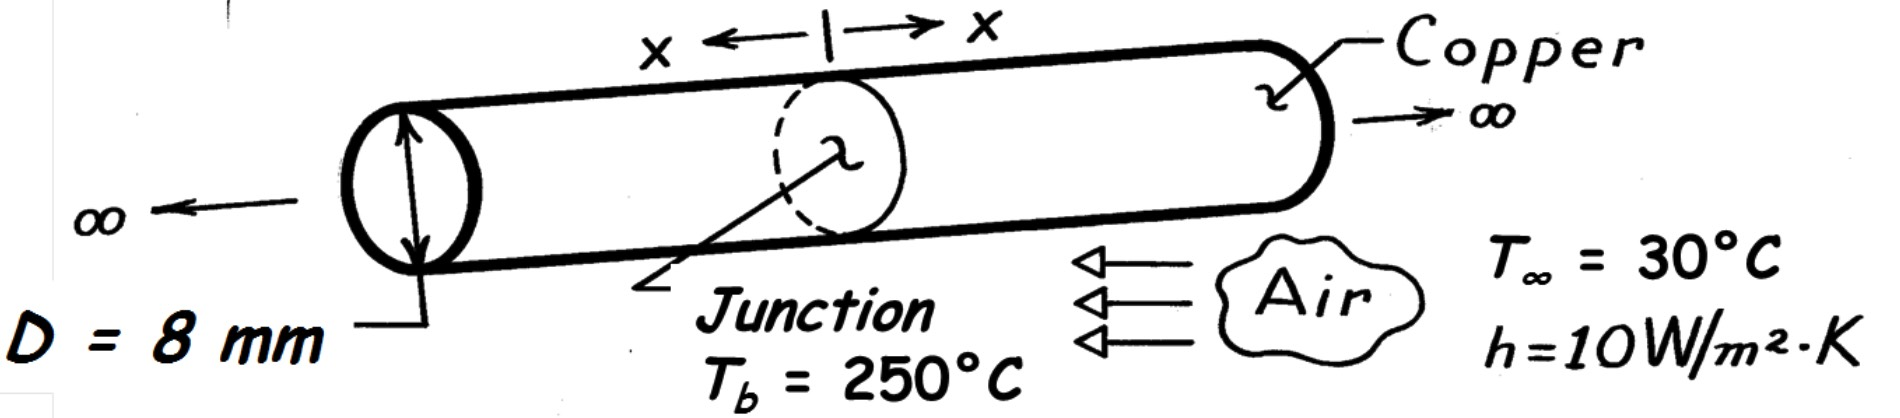
\includegraphics[width=0.95\textwidth]{Figures/fig2.1.jpg}
            \end{center}
        \end{figure}
        \vspace{2ex}
        \textbf{Note:}
        \begin{itemize}
            \item Use copper conductivity $k = \SI{379}{W/m.K}$
            \item The heat is directly input into the junction to solder the rods.
        \end{itemize}

    \end{columns}
\end{frame}

\begin{frame}{Problem 2 Solution}
    \begin{columns}
        \column{.8\textwidth}
        \textbf{3.136} Two long copper rods of diameter $D=\SI{10}{mm}$ are soldered together end to end, with solder having a melting point of \SI{650}{\degree C}. The rods are in air at \SI{25}{\degree C} with a convection coefficient of \SI{10}{W/m^2.K}. What is the \myhl{minimum power input} needed to effect the soldering?
        \vspace{2ex}

        \textbf{Solution:}
        \begin{itemize}
            \item The rod-junction-rod system can be treated as \myhl{infinite fin-junction-infinite fin}.
            \item The analytical solution to the infinite fin problem is:
                \begin{subequations}
                    \begin{alignat}{2}
                        &\text{Temperature:} &\quad & \theta/\theta_b = \exp(-m x) \\
                        &\text{Heat transfer rate} &\quad & q_f = M 
                    \end{alignat}
                \end{subequations}
                where $m = \sqrt{hP/kA_c}$, $M = \sqrt{hPkA_c}\theta_b$.
            \item Given that the junction temperature is \SI{650}{\degree C}, the corresponding power input should be:
                \begin{equation}
                    \begin{aligned}
                        q_{\text{min}} &= \myhl{2}q_f = 2M = 2\sqrt{hPkA_c}\theta_b \\
                        &= 2\sqrt{10\times (0.01\pi)\times 379\times (0.01^2\times \frac{\pi}{4})}\times (650-25) = \SI{120.9}{W}
                    \end{aligned}
                \end{equation}
        \end{itemize}
    \end{columns}
\end{frame}


\begin{frame}{Problem 3 (4.5 in the book)}
    \begin{columns}
        \column{0.3\textwidth}
        \begin{figure}
            \centering
            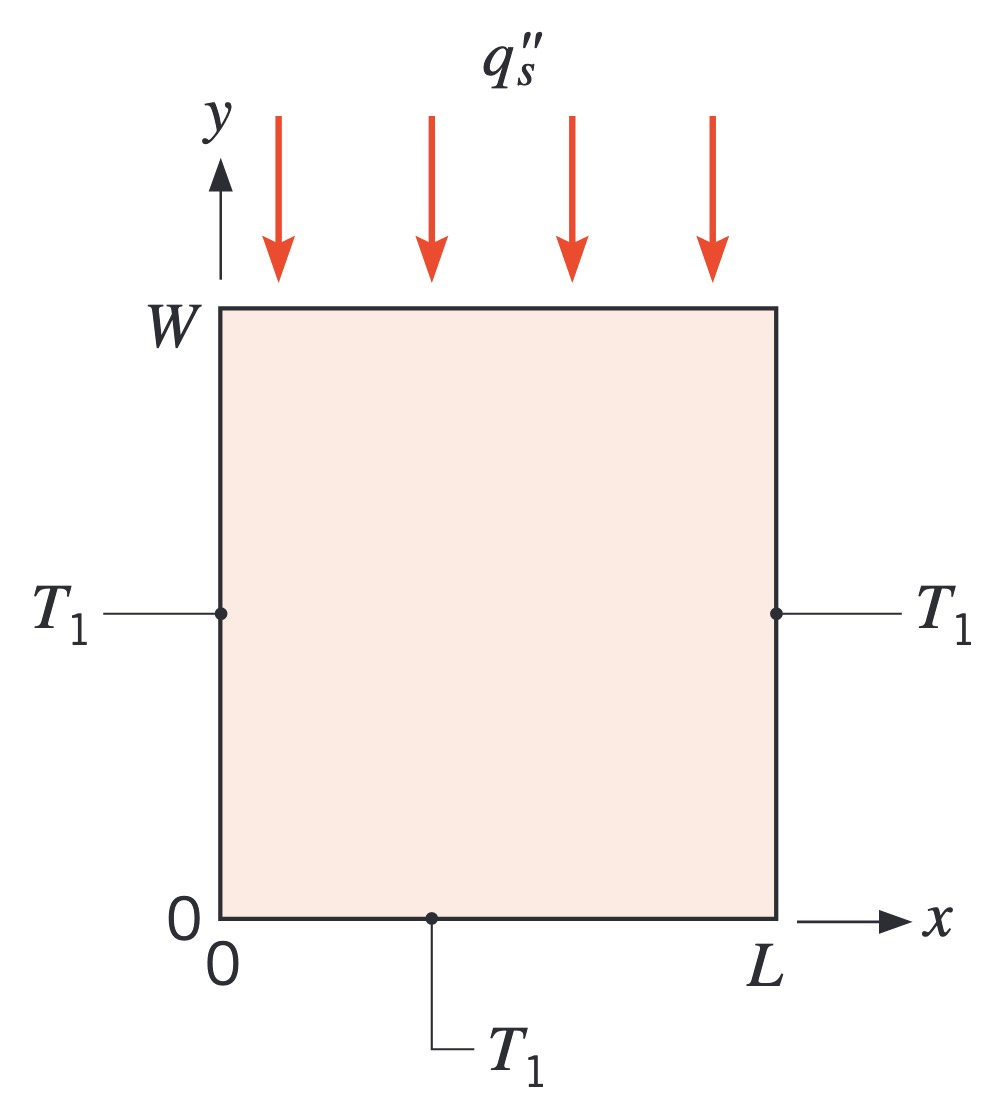
\includegraphics[width=1.0\textwidth]{Figures/fig2.2.jpg}
        \end{figure}
        \column{0.4\textwidth}
        \textbf{4.5} A two-dimensional rectangular plate is subjected to prescribed temperature boundary conditions on three sides and a uniform heat flux \textit{into} the plate at the top surface. Using the general approach of Section 4.2, derive an expression for the temperature distribution in the plate.
    \end{columns}
\end{frame}

\begin{frame}[allowframebreaks]{Problem 3 Solution}
    \textbf{4.5} A two-dimensional rectangular plate is subjected to prescribed temperature boundary conditions on three sides and a uniform heat flux \textit{into} the plate at the top surface. Using the general approach of Section 4.2, derive an expression for the temperature distribution in the plate.

    \vspace{2ex}
    \textbf{Solution:}
    Defining $\theta = T - T_1$, the heat equation and boundary conditions are:
    \begin{subequations}
        \begin{align}
            & \frac{\partial^2 \theta}{\partial x^2} + \frac{\partial^2 \theta}{\partial y^2} = 0 \label{eq:heat_2d}\\
            &\left\{ 
                \begin{alignedat}{2}
                    \theta (x=0, y) &= 0 &\quad &\text{(Left)} \\
                    \theta (x=L, y) &= 0 &\quad &\text{(Right)} \\
                    \theta (x, y=0) &= 0 &\quad &\text{(Bottom)} \\
                    -k\frac{\partial \theta}{\partial y}\Big|_{x, y=W} &= -q_s'' &\quad &\text{(Top)}
                \end{alignedat}
            \right.
        \end{align}
    \end{subequations}
    By seperation of variables, i.e., $\theta(x, y) = X(x)Y(y)$, Eq.~\eqref{eq:heat_2d} is modified to be,
    \begin{equation*}
        \frac{1}{X}\frac{\partial^2 X}{\partial x^2} = -\text{const}, \qquad
        \frac{1}{Y}\frac{\partial^2 Y}{\partial y^2} = \text{const}
    \end{equation*}
    with boundary conditions:
    \begin{equation*}
        X(0) = X(L) = Y(0) = 0, \quad -k X \frac{\mathrm{d} Y}{\mathrm{d} y}\Big|_{y=W} = -q_s''
    \end{equation*}

    \framebreak

    The constant value is either written as $-\beta^2$ or $\beta^2$ (with $\beta\geq 0$). If we choose $-\beta^2$, the solutions to $X$ and $Y$ are:
    \begin{equation*}
        X(x) = a_1 e^{\beta x} + a_2 e^{-\beta x}, \quad Y(y) = b_1 \sin(\beta y) + b_2 \cos(\beta y)
    \end{equation*}
    In this case, boundary conditions for $X(0)$ and $X(L)$ \myhl{cannot be satisfied} at the same time.
    Therefore, we take $\beta^2$ as the constant value, the general solution is thus:
    \begin{equation*}
        X(x) = a_1\sin(\beta x) + a_2\cos(\beta x), \quad Y(y) = b_1 e^{\beta y} + b_2 e^{-\beta y}
    \end{equation*}
    To meet the boundary conditions $X(0) = X(L) = 0$, we have $a_2 = 0$ and $\beta = n\pi/L$, with $n$ is a positive integer.
    For boundary condition $Y(0) = 0$, it is required that $b_2 = -b_1$, so that:
    \begin{equation*}
        X(x) = \sum_{n} A_n \sin\left(\frac{n\pi x}{L}\right), \quad Y(y) = \sum_n B_n \sinh\left(\frac{n\pi y}{L}\right)
    \end{equation*}
    Or,
    \begin{equation*}
        \theta(x) = \sum_n C_n \sin\left(\frac{n\pi x}{L}\right) \sinh\left(\frac{n\pi y}{L}\right)
    \end{equation*}
    where we combine the constants $A_n$ and $B_n$ into $C_n$.

    \framebreak

    The last boundary condition that we haven't used is the top surface:
    \begin{equation*}
        -k\frac{\partial \theta}{\partial y}\Big|_{x, y=W} = -q_s'' = -k\sum_n \myhl{C_n} \frac{n\pi}{L} \sin\left(\frac{n\pi \myhlb{x}}{L}\right) \cosh\left(\frac{n\pi W}{L}\right)
        \label{eq:top_surface}
    \end{equation*}
    See the book Eqs.~(4.14) to (4.16) for the solution to Eq.~\eqref{eq:top_surface}:
    \begin{subequations}
        \begin{align}
            f(x) &= \sum_n A_n g_n (x) \tag{4.14 in the book} \\
            A_n &= \frac{\int_a^b f(x)g_n(x)\mathrm{d}x}{\int_a^b g_n^2(x)\mathrm{d}x} \tag{4.16 in the book}
        \end{align}
    \end{subequations}
    Here, the ``$C_n$'' is the ``$A_n$'' in the book, ``$\frac{q_s''L}{kn\pi\cosh(n\pi W/L)}$'' is the ``$f(x)$'' in the book, and $g_n (x) = \sin(n\pi x/L)$, therefore
    \begin{equation*}
        C_n = 2\frac{q_s''L}{kn^2 \pi^2 \cosh(n\pi W/L)} \left[(-1)^{n+1} + 1 \right]
    \end{equation*}
\end{frame}

\end{document}
